\documentclass[mathserif,11pt]{beamer}

\usepackage{url,verbatim,natbib}
\usepackage[english]{babel}
\usepackage{amsmath, mathabx}
\usepackage{dsfont, ulem}
\usepackage{tikz}
\usepackage{xparse}
\newtheorem{proposition}[theorem]{Proposition}

\usepackage[headheight=22pt]{beamerthemeboxes}
\usepackage{graphicx}
\beamertemplatenavigationsymbolsempty 
\setbeamercovered{transparent}
\usepackage{centernot}

\setbeamertemplate{itemize item}{$\bullet$} 
\setbeamercolor{title}{fg=uio}
\setbeamertemplate{sections/subsections in toc}[ball unnumbered]
\setbeamercolor{section in toc}{fg=uio,bg=white}
\setbeamercolor{subsection in toc}{fg=uio,bg=white}
\setbeamercolor{result}{fg=black, bg=yellow}
\newcommand{\dotsim}{\stackrel{\cdot}{\sim}}
\newcommand{\interi}{{\rm Z}\negthinspace\negthinspace {\rm Z}}
\newcommand{\reali}{{\rm I}\negthinspace {\rm R}}
\newcommand{\naturali}{{\rm I}\negthinspace {\rm N}}
\newcommand{\sign}{\mathop{\rm sgn}\nolimits}
\newcommand{\sgn}{\mathop{\mathrm{sgn}}}
\definecolor{redve}{rgb}{0.604,0.008,0.00}
\definecolor{lmu}{rgb}{0.188,0.522,0.306}
\definecolor{uio}{rgb}{0.847,0.118,0.02}

\def\R{{\rm I\!R}}
\def\P{{\rm Pr}}
\def\Real{{\rm I\!R}}
\def\T{{\footnotesize {^{_{\sf T}}}}}
\def\tr{{\rm tr}}
\def\diag{{\rm diag}}

\NewDocumentCommand\DownArrow{O{2.0ex} O{black}}{%
   \mathrel{\tikz[baseline] \draw [<-, line width=0.5pt, #2] (0,0) -- ++(0,#1);}
}

\useframetitletemplate{% 
\begin{centering} 
\begin{small} \structure{\textcolor{uio} \insertframetitle {\insertframesubtitle}}
\end{small}

\end{centering} 
}

\addheadboxtemplate{\color[rgb]{1,1,1}}{\color{uio} \underline{{\hspace{5pt}\includegraphics[scale=0.06]{../../../../support/uio_logo_eng} \hspace{0.265\paperwidth}\color{black} \tiny  STK-IN4300 - Statistical Learning Methods in Data Science} \hspace{5pt}}}

%\bfseries{\insertsection}

\addfootboxtemplate{\color[rgb]{1,1,1}}{\color{black} \tiny \quad  
STK-IN4300: lecture 11
  \hfill \tiny \insertframenumber / \inserttotalframenumber \hspace{5pt}}

  
\title{STK-IN4300 \\ Statistical Learning Methods in Data Science}
\author{Riccardo De Bin} 
\institute{debin@math.uio.no} 
\date{}


\begin{document}
\setbeamercolor{bgr}{fg=black,bg=uio}

{
\setbeamertemplate{headline}{}
\frame{
\vspace{-2cm}
\begin{beamercolorbox}[sep=-2.2em,wd=5cm,colsep=0.5pt,ht=4.25ex,dp=3ex,left]{postit}
\includegraphics[scale=0.06]{../../../../support/uio_logo_eng}
\end{beamercolorbox}
\vspace{0.365cm}
\noindent\makebox[\linewidth]{\color{uio} \rule{\paperwidth}{0.4pt}}
\vspace{2.5cm}
\titlepage
}
}

\frame{\frametitle{Outline of the lecture}
\tableofcontents
}


\section{Gradient Boosting}

\subsection{review}

\frame{\frametitle{Gradient Boosting: }
\framesubtitle{from the last lecture}
In the last lecture:
\begin{itemize}
\item boosting as implementation of \textcolor{uio}{``wisdom of the crowds''};
\item \textcolor{uio}{repeatedly} apply a \textcolor{uio}{weak learner} to modification of the data;
\item from \textcolor{uio}{AdaBoost} to \textcolor{uio}{gradient boosting};
\item forward stagewise additive modelling;
\item importance of \textcolor{uio}{shrinkage}.
\end{itemize}
}


\frame{\frametitle{Gradient Boosting: }
\framesubtitle{general gradient boosting}
The general algorithm for the \textcolor{uio}{gradient boosting}:
\begin{enumerate}
\setlength\itemsep{5pt}
\item \textcolor{uio}{initialize} the estimate, e.g., $f_0(x) = 0$;
\item for $m = 1, \dots, m_\text{stop}$,
\begin{itemize}
\setlength\itemsep{5pt}
  \item[2.1] compute the \textcolor{uio}{negative gradient} vector, $u_m=-\left.\frac{\partial L(y,f(x))}{\partial f(x)}\right|_{f(x)=\hat{f}_{m-1}(x)}$;
  \item[2.2] fit the \textcolor{uio}{base learner} to the negative gradient vector, $h_m(u_m,x)$;
  \item[2.3] \textcolor{uio}{update} the estimate, $f_m(x) = f_{m-1}(x) + \nu h_m(u_m,x)$.
\end{itemize}
\item \textcolor{uio}{final} estimate, $\hat{f}_{m_\text{stop}}(x) = \sum_{m=1}^{m_\text{stop}} \nu h_m(u_m,x)$
\end{enumerate}
}


\subsection{L$_2$ boosting with linear learner}

\frame{\frametitle{Gradient Boosting: }
\framesubtitle{L$_2$ boosting with linear learner}
The \textcolor{uio}{$L_2$Boost} algorithm (linear learner, L$_2$ loss):
\begin{enumerate}
\setlength\itemsep{5pt}
\item initialize the estimate, e.g., $\hat{\beta}_0 = 0$;
\item for $m = 1, \dots, m_\text{stop}$,
\begin{itemize}
\setlength\itemsep{5pt}
  \item[2.1] compute the \textcolor{uio}{negative gradient vector}, $u_m=-\left.\frac{\partial L(y,f(X,\beta))}{\partial f(X,\beta)}\right|_{\beta=\hat{\beta}_{m-1}}$;
  \item[2.2] fit the \textcolor{uio}{base learner} to the negative gradient vector, $b_m(u_m,X) = \nu (X^TX)^{-1}X^Tu_m$;
  \item[2.3] update the estimate, $\hat{\beta}_m = \hat{\beta}_{m-1} + b_m(u_m,x)$.
\end{itemize}
\item final estimate, $\hat{f}_{m_\text{stop}}(x) = X^T\hat{\beta}_m$.
\end{enumerate}
}


\frame{\frametitle{L$_2$ boosting with linear learner: }
\framesubtitle{boosting operator}
Consider the regression model $y_i = f(x_i) + \epsilon_i$, $i = 1, \dots, N$,
\begin{itemize}
\item $\epsilon_i$ i.i.d.\ with $E[\epsilon_i]=0$, $\text{Var}[\epsilon_i]=\sigma^2$.
\item linear learner $\mathcal{S}: \mathds{R}^N \rightarrow \mathds{R}^N$ ($\mathcal{S}y = \hat{y}$);
\end{itemize}

\vspace{6pt}

Note that:
\begin{itemize}
\item $\hat{f}_m(x) = \hat{f}_{m-1}(x) + \mathcal{S}u_m$;
\item $u_m = y - \hat{f}_{m-1}(x) = u_{m-1} - \mathcal{S}u_{m-1} = (I - \mathcal{S})u_{m-1}$;
\item iterating, \textcolor{uio}{$u_m = (I - \mathcal{S})^m$}, $m = 1, \dots, m_\text{stop}$.
\end{itemize}

\vspace{6pt}

Because $\hat{f}_m(x) = \mathcal{S}y$, then $\hat{f}_{m_\text{stop}}(x) = \sum_{m=0}^{m_\text{stop}} \mathcal{S}(I - \mathcal{S})^m y$, i.e.,
$$
\hat{f}_{m_\text{stop}}(x) = \underbrace{(I - (I - \mathcal{S})^{m+1})}_{\textcolor{uio}{\text{boosting operator } \mathcal{B}_m}}y.
$$
}


\frame{\frametitle{L$_2$ boosting with linear learner: }
\framesubtitle{properties}
Consider a \textcolor{uio}{linear} learner $\mathcal{S}$ (e.g., least square). Then

\vspace{6pt}

{\it Proposition 1 \citep{BuehlmannYu2003}:} The \textcolor{uio}{eigenvalues} of the \textcolor{uio}{$L_2$Boost operator $\mathcal{B}_m$} are
$$
\left\{1-(1-\lambda_k)^{m_\text{stop}+1}, k = 1, \dots, N\right\}.
$$

If $\mathcal{S} = \mathcal{S}^T$ (i.e., symmetric), then \textcolor{uio}{$\mathcal{B}_m$ can be diagonalized} with an orthonormal transformation,
$$
\mathcal{B}_m = UD_mU^T, \quad\quad D_m = \text{diag}(1-(1-\lambda_k)^{m_\text{stop}+1})
$$
where $U U^T = U^T U = I$.
}


\frame{\frametitle{L$_2$ boosting with linear learner: }
\framesubtitle{properties}
We can now compute:
\begin{itemize} 
\item $\text{bias}^2(m, \mathcal{S}; f) \begin{aligned}[t] &= N^{-1}\sum_{i = 1}^N (E[\hat{f}_m(x_i)] - f)^2 \\
&= N^{-1} f^T U \text{diag}(\textcolor{uio}{(1-\lambda_k)^{2m+2}})U^Tf;
\end{aligned}$
\item $\text{Var}(m, \mathcal{S}; \sigma^2) \begin{aligned}[t] &= N^{-1}\sum_{i = 1}^N (\text{Var}[\hat{f}_m(x_i)]) \\
&= \sigma^2N^{-1}\sum_{i = 1}^N \textcolor{uio}{(1-(1-\lambda_k)^{m+1})^2};
\end{aligned}$
\end{itemize}
and
\begin{itemize} 
\item $\text{MSE}(m,\mathcal{S}; f, \sigma^2) = \text{bias}^2(m, \mathcal{S}; f) + \text{Var}(m, \mathcal{S}; \sigma^2)$.
\end{itemize}
}


\frame{\frametitle{L$_2$ boosting with linear learner: }
\framesubtitle{properties}
Assuming $0 < \lambda_k \leq 1$, $k = 1, \dots, N$, note that:
\begin{itemize}
\setlength\itemsep{5pt}
\item $\text{bias}^2(m, \mathcal{S}; f)$ \textcolor{uio}{decays exponentially} fast for $m$ increasing;
\item $\text{Var}(m, \mathcal{S}; \sigma^2)$ \textcolor{uio}{increases exponentially slow} for $m$ increasing;
\item \textcolor{uio}{$\lim_{m\rightarrow \infty} \text{MSE}(m,\mathcal{S}; f, \sigma^2) = \sigma^2$};
\item if \textcolor{uio}{$\exists k: \lambda_k < 1$} (i.e., $\mathcal{S} \neq I$), then \textcolor{uio}{$\exists m : \text{MSE}(m,\mathcal{S}; f, \sigma^2) < \sigma^2$};
\item if \textcolor{uio}{$\forall k: \lambda_k<1, \frac{\mu_k}{\sigma^2} > \frac{1}{(1-\lambda_k)^2} - 1$}, then \textcolor{uio}{$MSE_{\mathcal{B}_m} < MSE_{\mathcal{S}}$},
where $\mu=U^Tf$ ($\mu$ represents $f$ in the coordinate system of the eigenvectors of $\mathcal{S}$).
\item[]
\end{itemize}
\cite[for the proof, see][Theorem 1]{BuehlmannYu2003}
}


\frame{\frametitle{L$_2$ boosting with linear learner: }
\framesubtitle{properties}
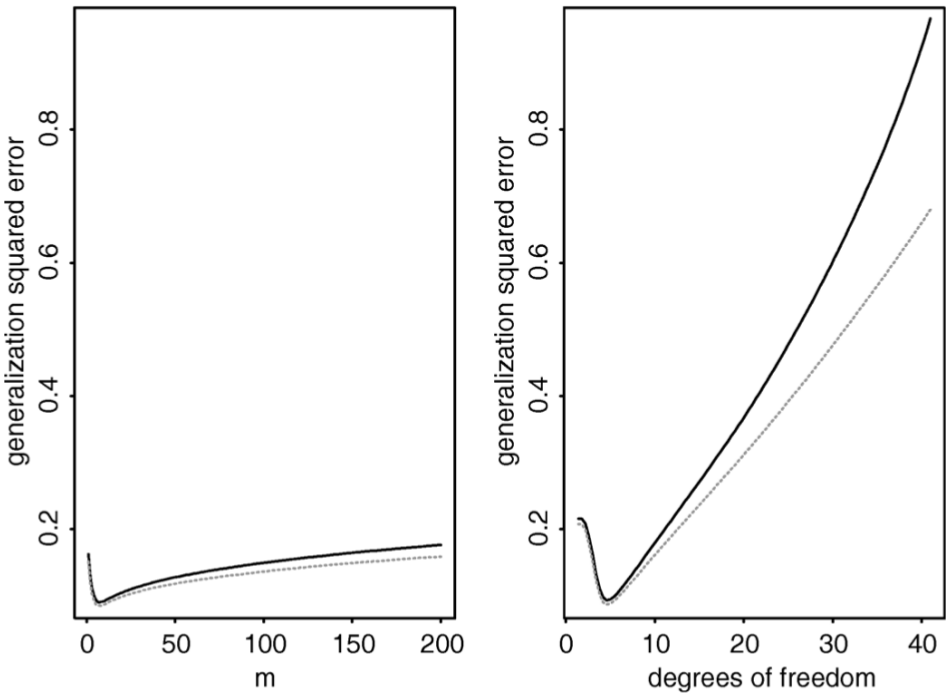
\includegraphics[width=0.965\textwidth]{fig1_by}
}


\frame{\frametitle{L$_2$ boosting with linear learner: }
\framesubtitle{properties}
About $\frac{\mu_k}{\sigma^2} > \frac{1}{(1-\lambda_k)^2} - 1$:
\begin{itemize}
\item a large left side means that \textcolor{uio}{$f$ is relatively complex compared} with the noise level \textcolor{uio}{$\sigma^2$};
\item a small right side means that $\lambda_k$ is small, i.e.\ the learner \textcolor{uio}{shrinks strongly} in the direction of the $k$-th eigenvector;
\item therefore, to have boosting bringing improvements:
\begin{itemize}
\item there must be a \textcolor{uio}{large} signal to noise ratio;
\item the value of $\lambda_k$ must be \textcolor{uio}{sufficiently small};
\end{itemize}
\item[] \centering $\downarrow$
\item[] use a \textcolor{uio}{weak learner}!!!
\end{itemize}
}


\frame{\frametitle{L$_2$ boosting with linear learner: }
\framesubtitle{properties}
There is a further intersting theorem in \cite{BuehlmannYu2003},

\vspace{12pt}

{\it Theorem 2:} Under the assumption seen till here and $0 < \lambda_k \leq 1$, $k = 1, \dots, N$, and assuming that $E[|\epsilon_1|^p] < \infty$ for $p \in \mathds{N}$,
$$
N^{-1} \sum_{i = 1}^N E[(\hat{f}_m(x_i) - f(x_i))^p] = E[\epsilon_1^p] + \textcolor{uio}{O(e^{-Cm})},\quad m\rightarrow \infty
$$
where $C>0$ does not depend on $m$ (but on $N$ and $p$).

\vspace{12pt}

This theorem can be used to argue that boosting for classification is \textcolor{uio}{resistant to overfitting} (for $m\rightarrow \infty$, exponentially small overfitting).
}


\frame{\frametitle{Gradient Boosting: }
\framesubtitle{boosting in high-dimensions}
The boosting algorithm is working in \textcolor{uio}{high-dimension frameworks}:
\begin{itemize}
\item forward stagewise additive modelling;
\item at each step, \textcolor{uio}{only one dimension} (component) of X is updated at each iteration;
\item in a \textcolor{uio}{parametric} setting, only one $\hat{\beta}_j$ is updated;
\item an additional step in which it is decided \textcolor{uio}{which component to update} must be computed at each iteration.
\end{itemize}
}


\frame{\frametitle{Gradient Boosting: }
\framesubtitle{component-wise L$_2$Boost with linear learner}
{\bf \uline{Component-wise L$_2$Boost algorithm}:}
\begin{enumerate}
\item initialize the estimate, e.g., $\hat{\beta} = (0,\dots,0)$;
\item for $m = 1, \dots, m_\text{stop}$,
\begin{itemize}
\item compute the negative gradient vector, $u=-\left.\frac{\partial L(y,f(x,\beta))}{\partial f(x,\beta)}\right|_{\beta=\hat{\beta}}$ for the \textcolor{uio}{$j$-th component only};
\item fit the base learner to the negative gradient vector, $\hat{h}(u,x_j)$;
\item \textcolor{uio}{select the best update $j^*$} (usually that minimizes the loss);
\item include the shrinkage factor, $\hat{b}_j=\nu\hat{h}(u,x_j)$;
\item update the estimate, $\hat{\beta}_{j^*} = \hat{\beta}_{j^*} + \hat{b}_{j^*}$.
\end{itemize}
\item final estimate, $\hat{f}_{m_\text{stop}}(x) = X^T\hat{\beta}^{[m_\text{stop}]}$ (for linear regression).
\end{enumerate}
}


\frame{\frametitle{Boosting: }
\framesubtitle{minimization of the loss function}
\vspace{-0.75cm}
\begin{figure}
  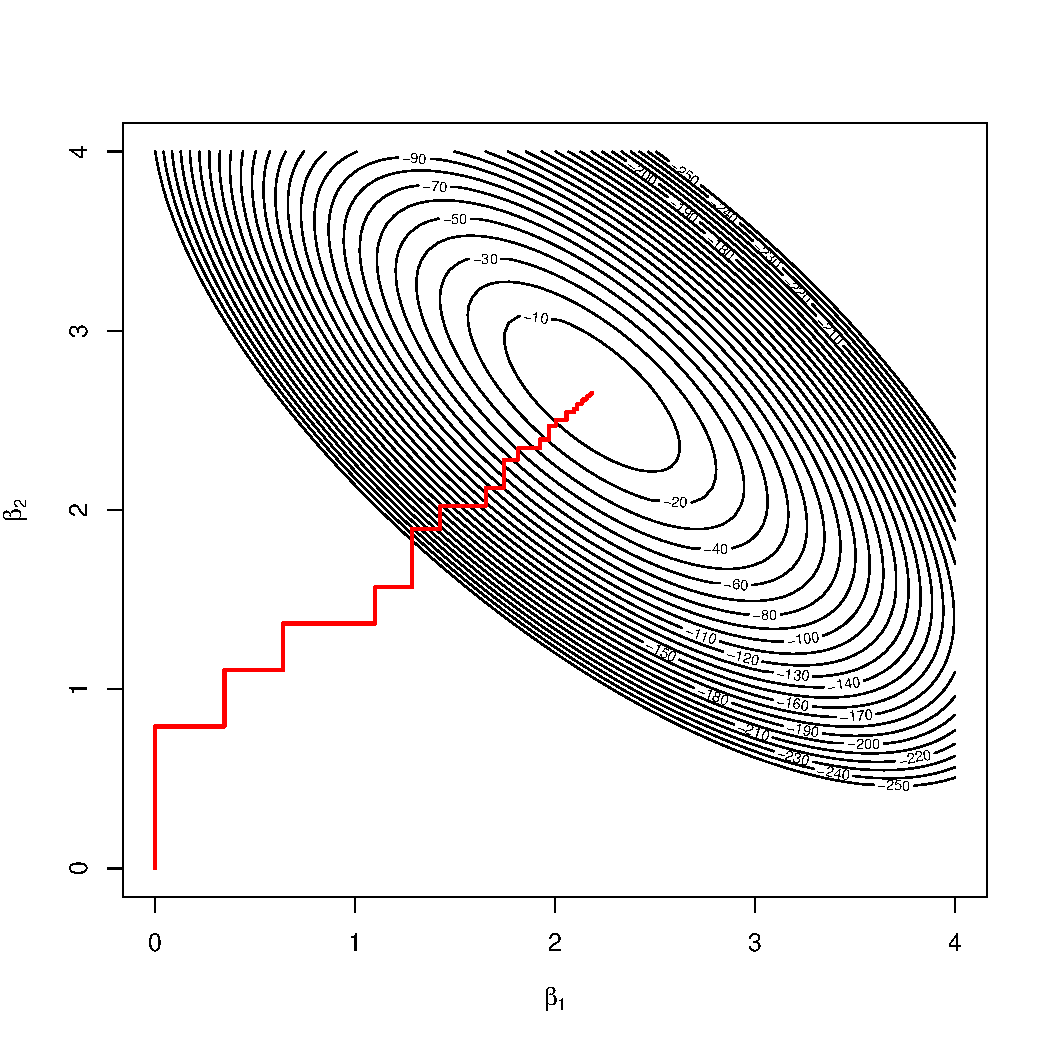
\includegraphics[width=0.75\textwidth]{figures/figure_llik}
\end{figure}
}


\frame{\frametitle{Boosting: }
\framesubtitle{parameter estimation}
\vspace{-0.75cm}
\begin{figure}
  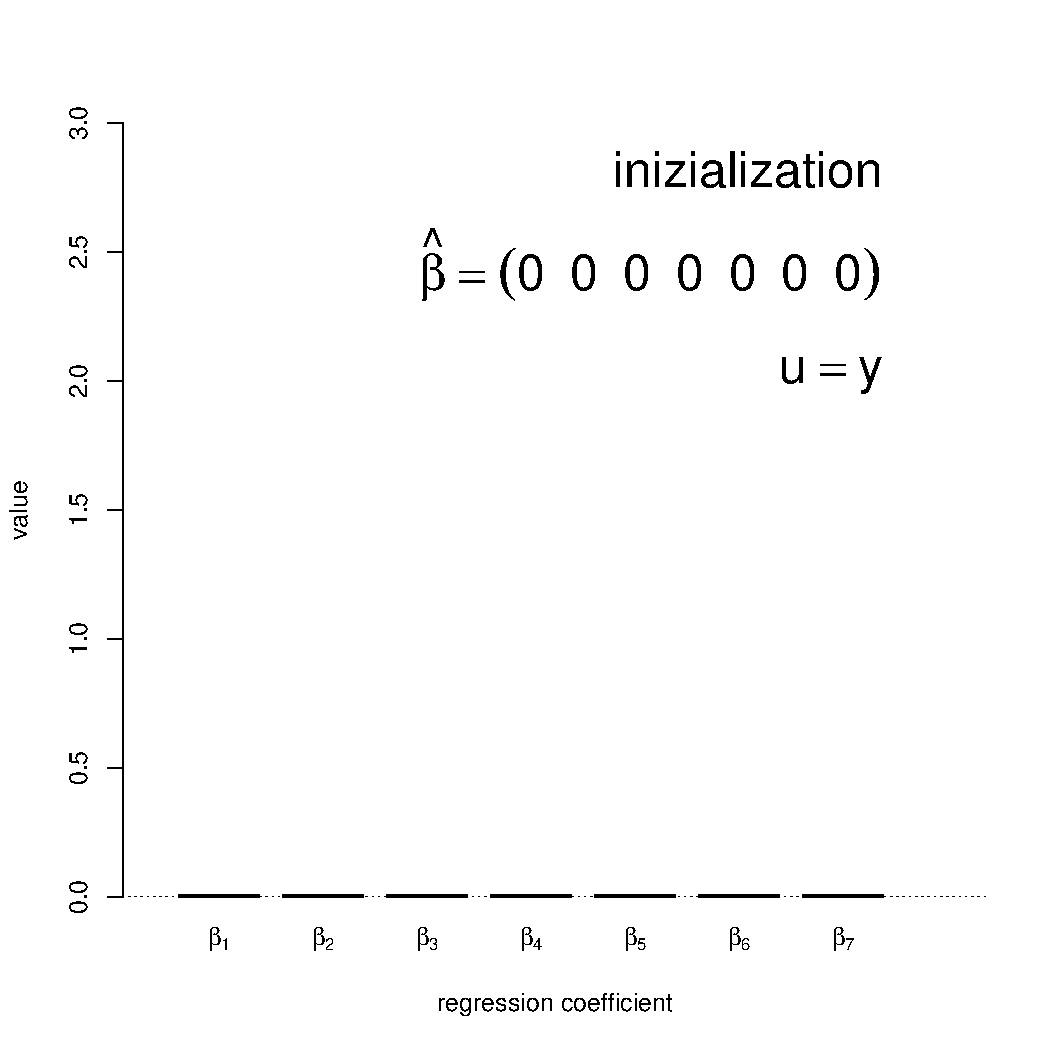
\includegraphics[width=0.75\textwidth]{figures/boosting_0}
\end{figure}
}

\frame{\frametitle{Boosting: }
\framesubtitle{parameter estimation}
\vspace{-0.75cm}
\begin{figure}
  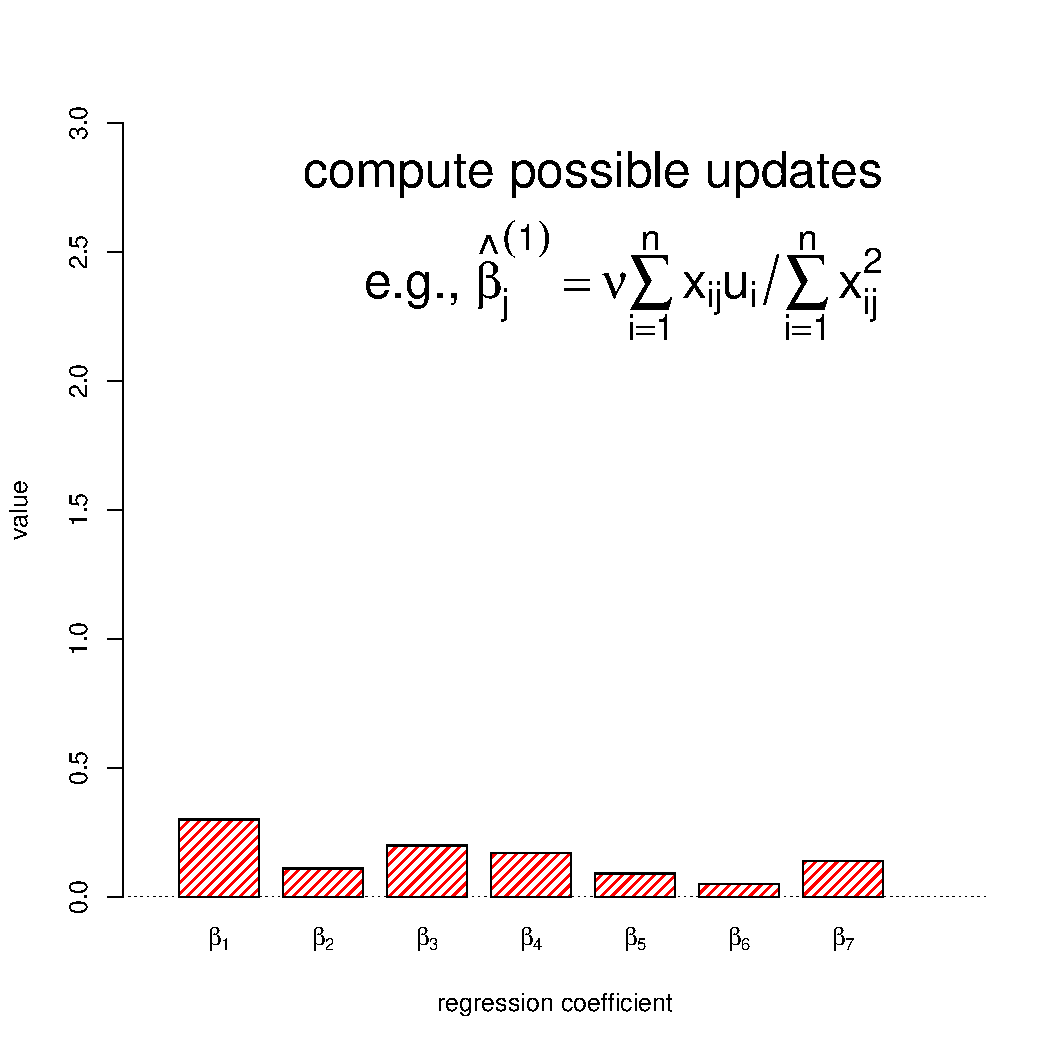
\includegraphics[width=0.75\textwidth]{figures/boosting_1}
\end{figure}
}

\frame{\frametitle{Boosting: }
\framesubtitle{parameter estimation}
\vspace{-0.75cm}
\begin{figure}
  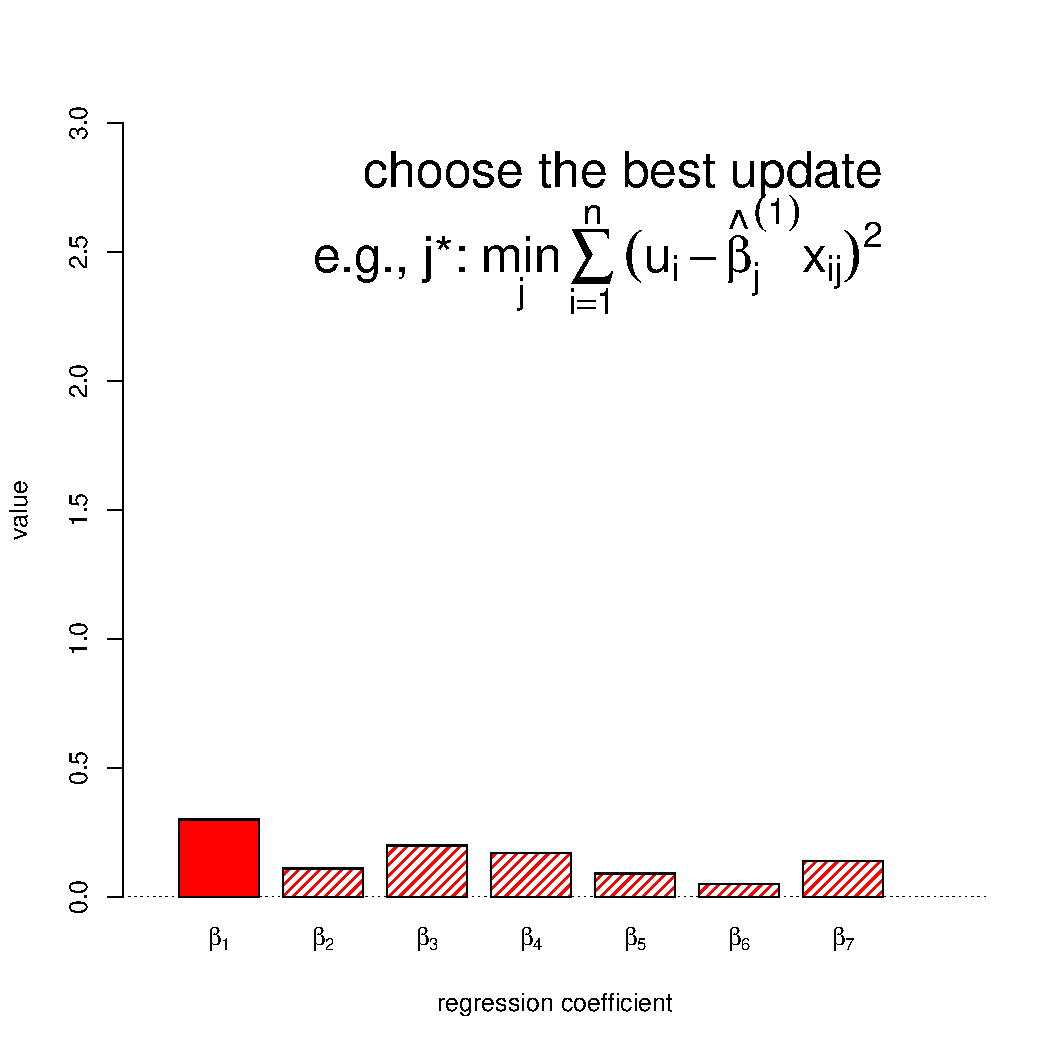
\includegraphics[width=0.75\textwidth]{figures/boosting_2}
\end{figure}
}

\frame{\frametitle{Boosting: }
\framesubtitle{parameter estimation}
\vspace{-0.75cm}
\begin{figure}
  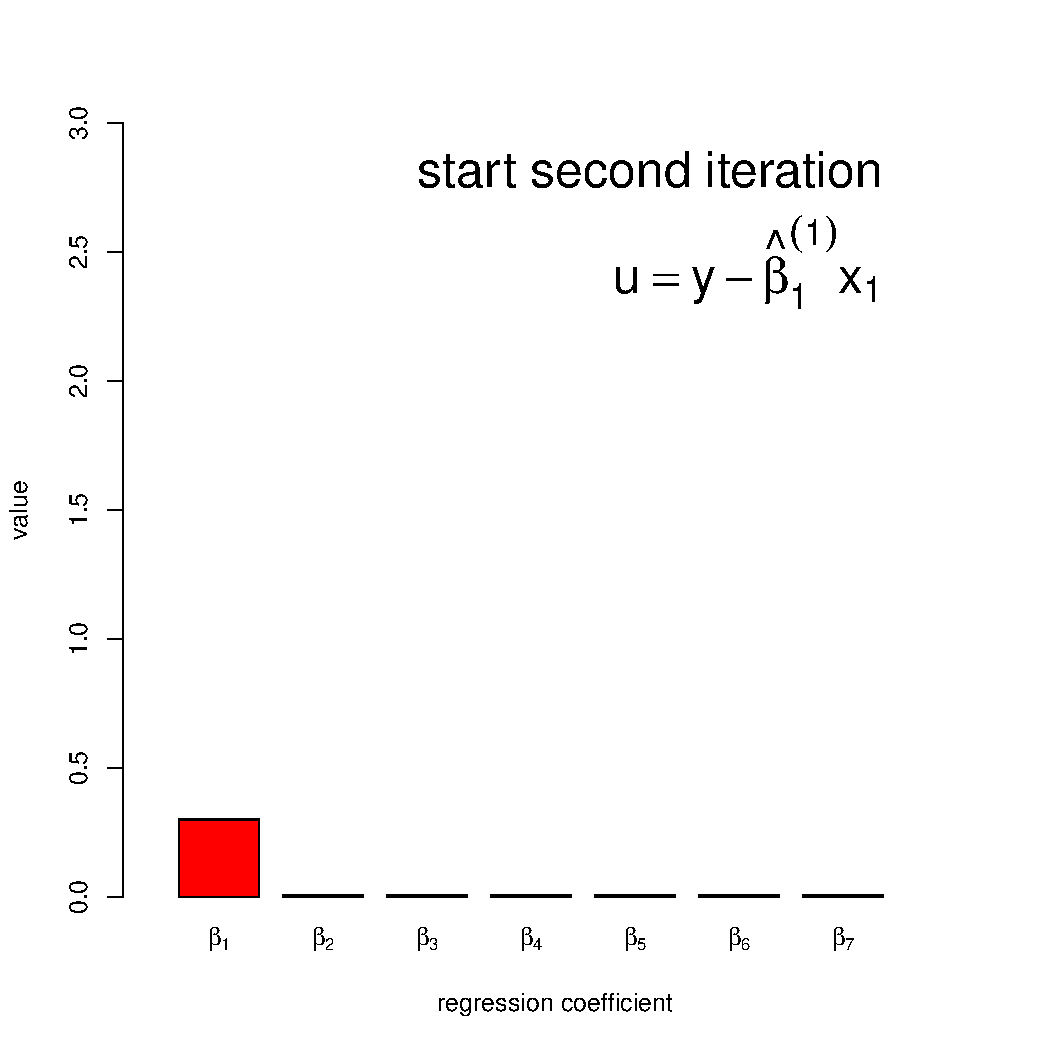
\includegraphics[width=0.75\textwidth]{figures/boosting_3}
\end{figure}
}

\frame{\frametitle{Boosting: }
\framesubtitle{parameter estimation}
\vspace{-0.75cm}
\begin{figure}
  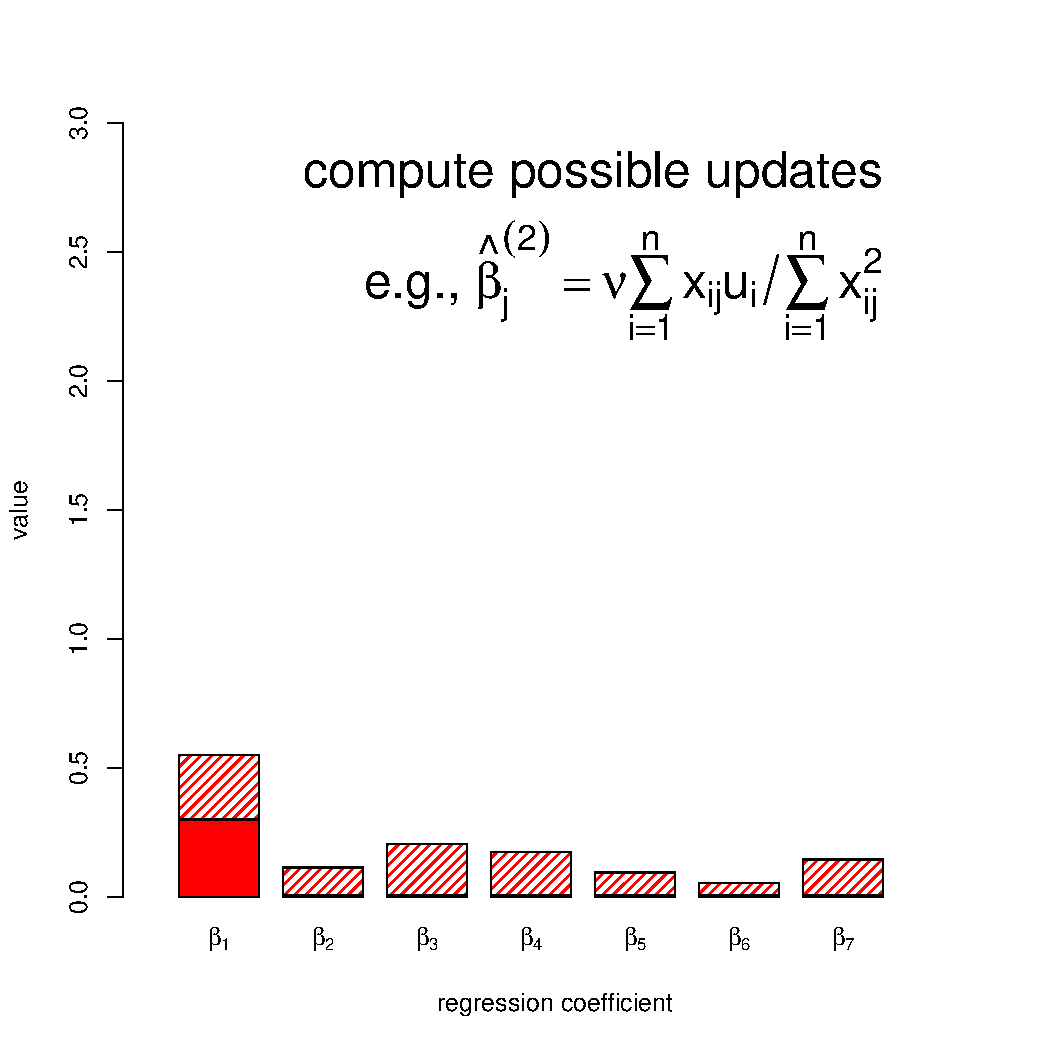
\includegraphics[width=0.75\textwidth]{figures/boosting_4}
\end{figure}
}

\frame{\frametitle{Boosting: }
\framesubtitle{parameter estimation}
\vspace{-0.75cm}
\begin{figure}
  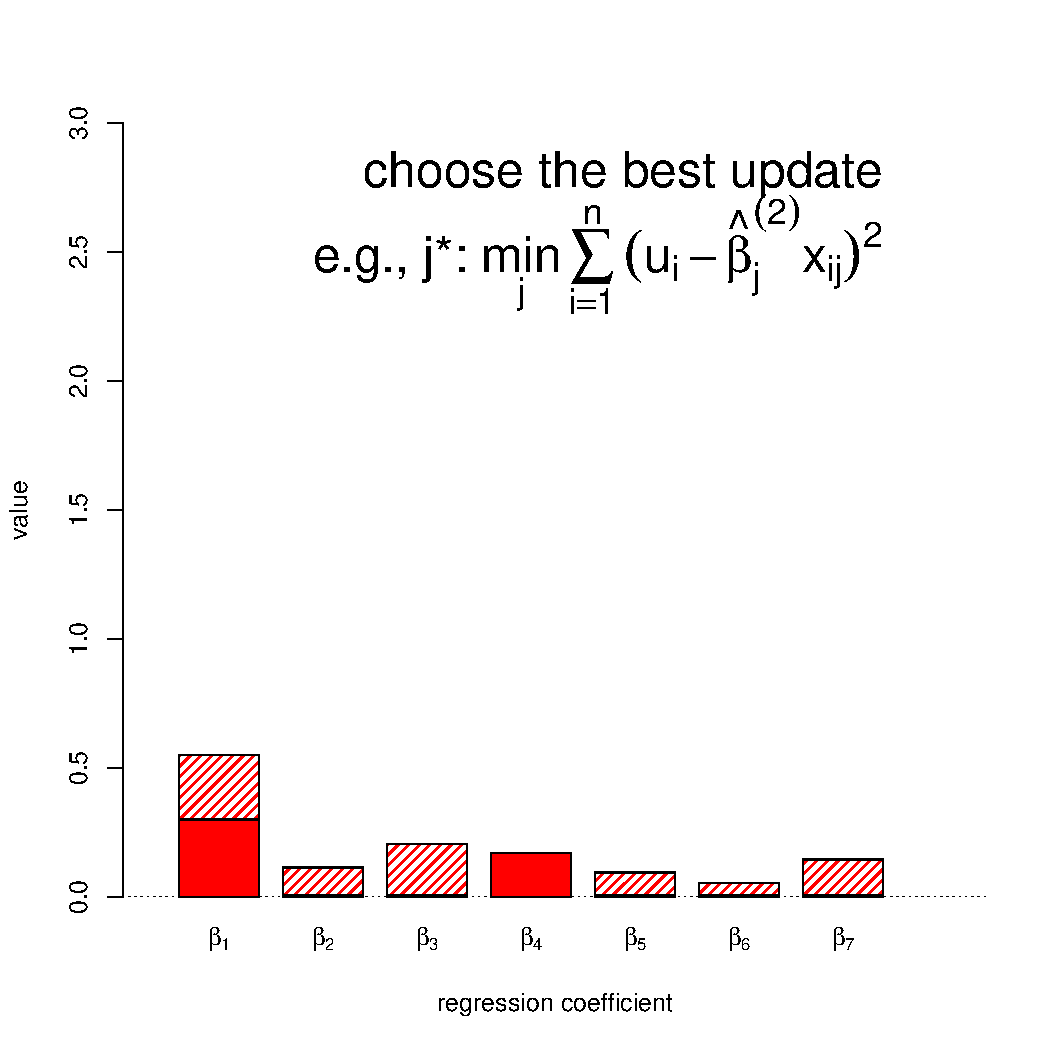
\includegraphics[width=0.75\textwidth]{figures/boosting_5}
\end{figure}
}

\frame{\frametitle{Boosting: }
\framesubtitle{parameter estimation}
\vspace{-0.75cm}
\begin{figure}
  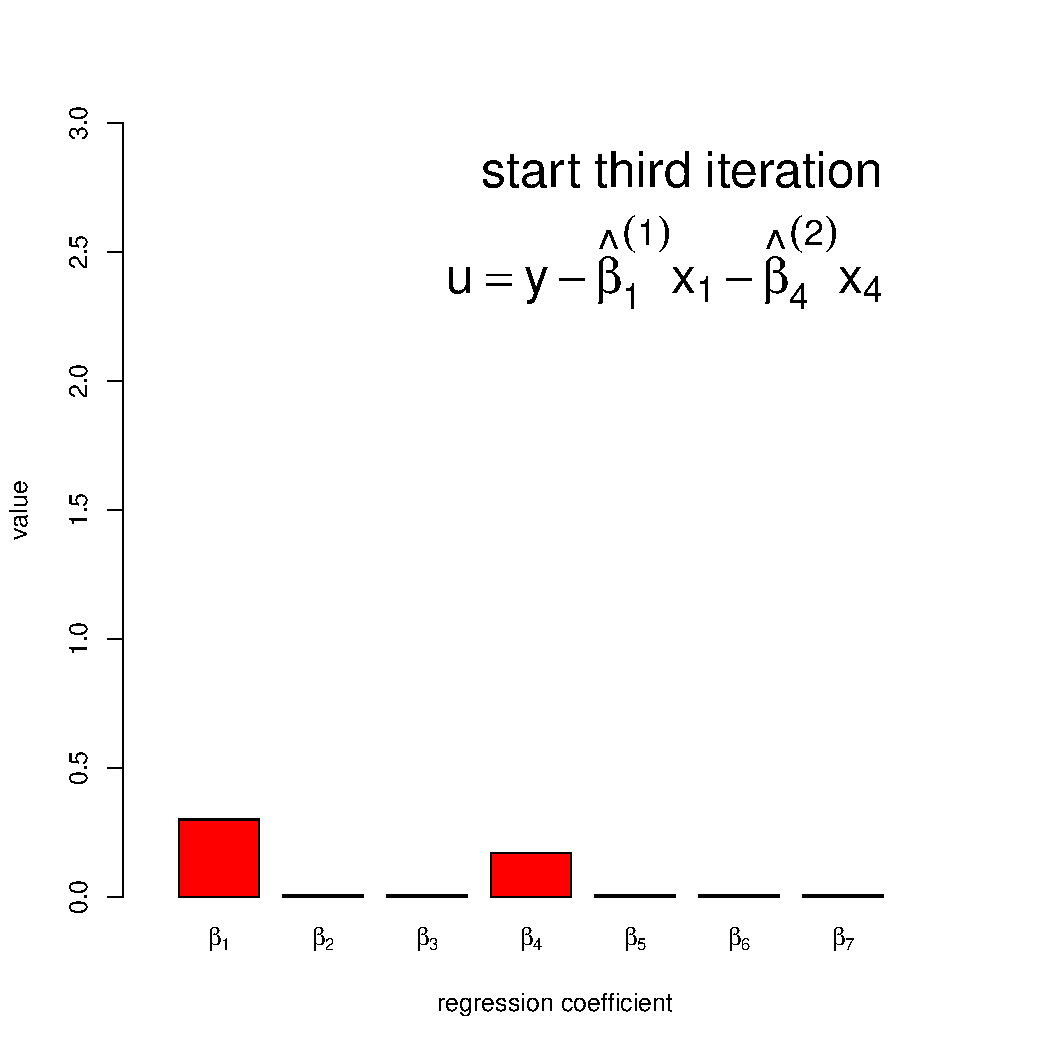
\includegraphics[width=0.75\textwidth]{figures/boosting_6}
\end{figure}
}

\frame{\frametitle{Boosting: }
\framesubtitle{parameter estimation}
\vspace{-0.75cm}
\begin{figure}
  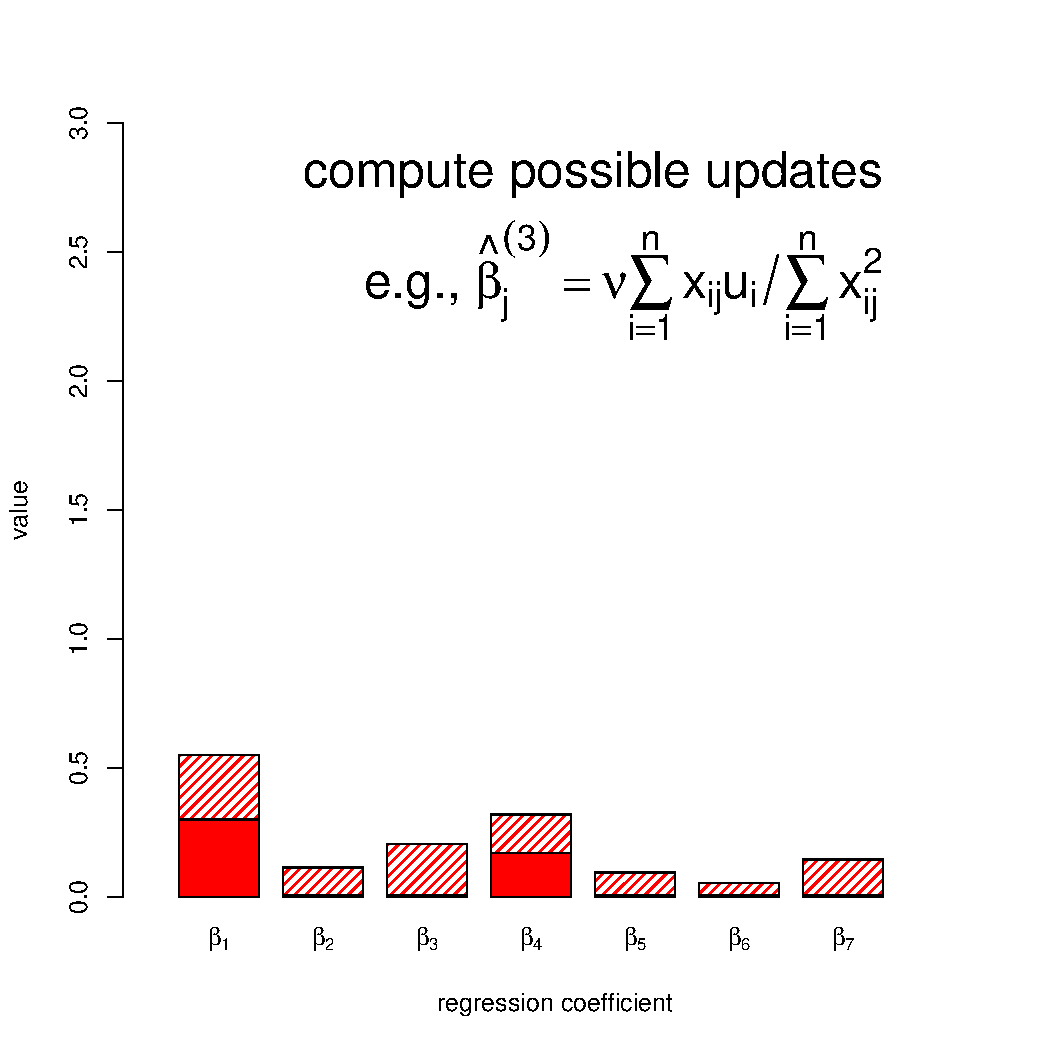
\includegraphics[width=0.75\textwidth]{figures/boosting_7}
\end{figure}
}

\frame{\frametitle{Boosting: }
\framesubtitle{parameter estimation}
\vspace{-0.75cm}
\begin{figure}
  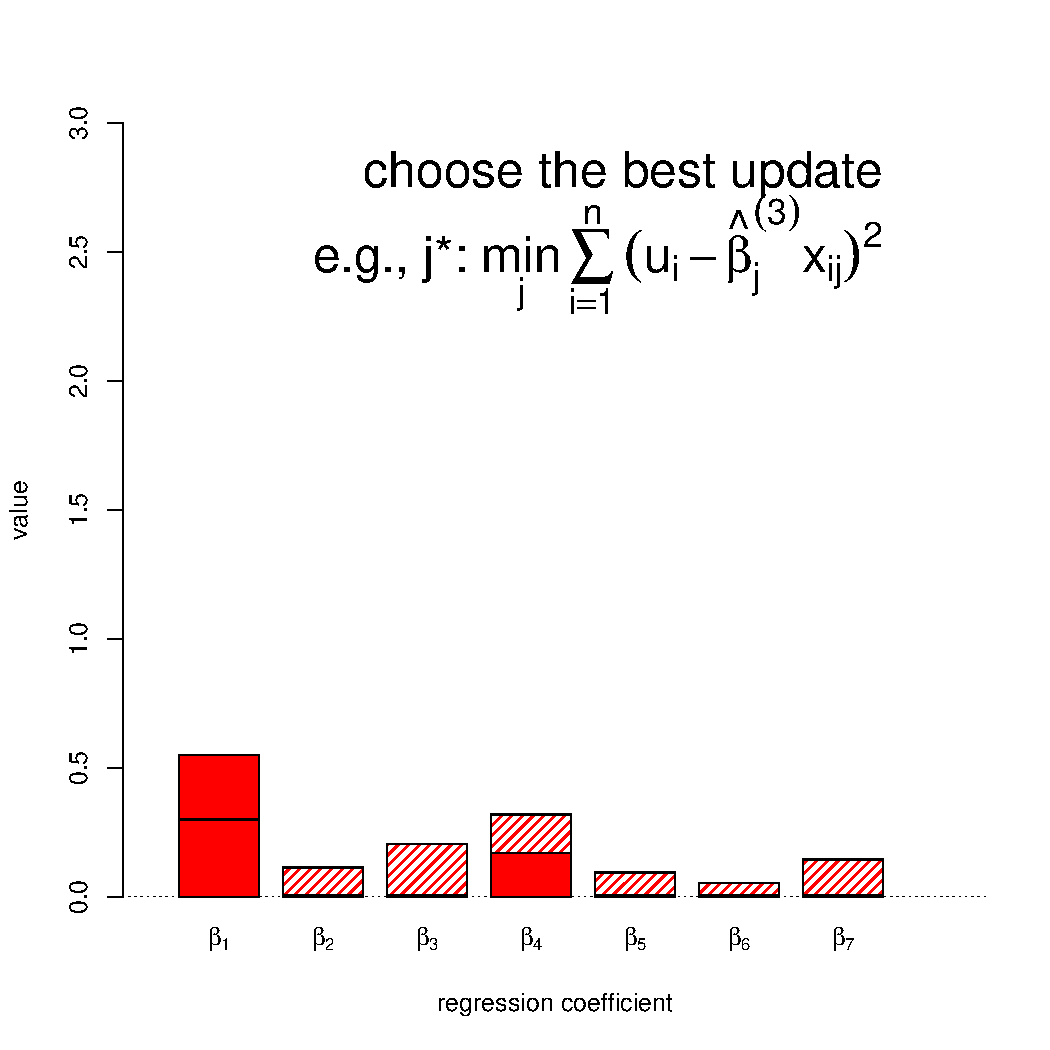
\includegraphics[width=0.75\textwidth]{figures/boosting_8}
\end{figure}
}

\frame{\frametitle{Boosting: }
\framesubtitle{parameter estimation}
\vspace{-0.75cm}
\begin{figure}
  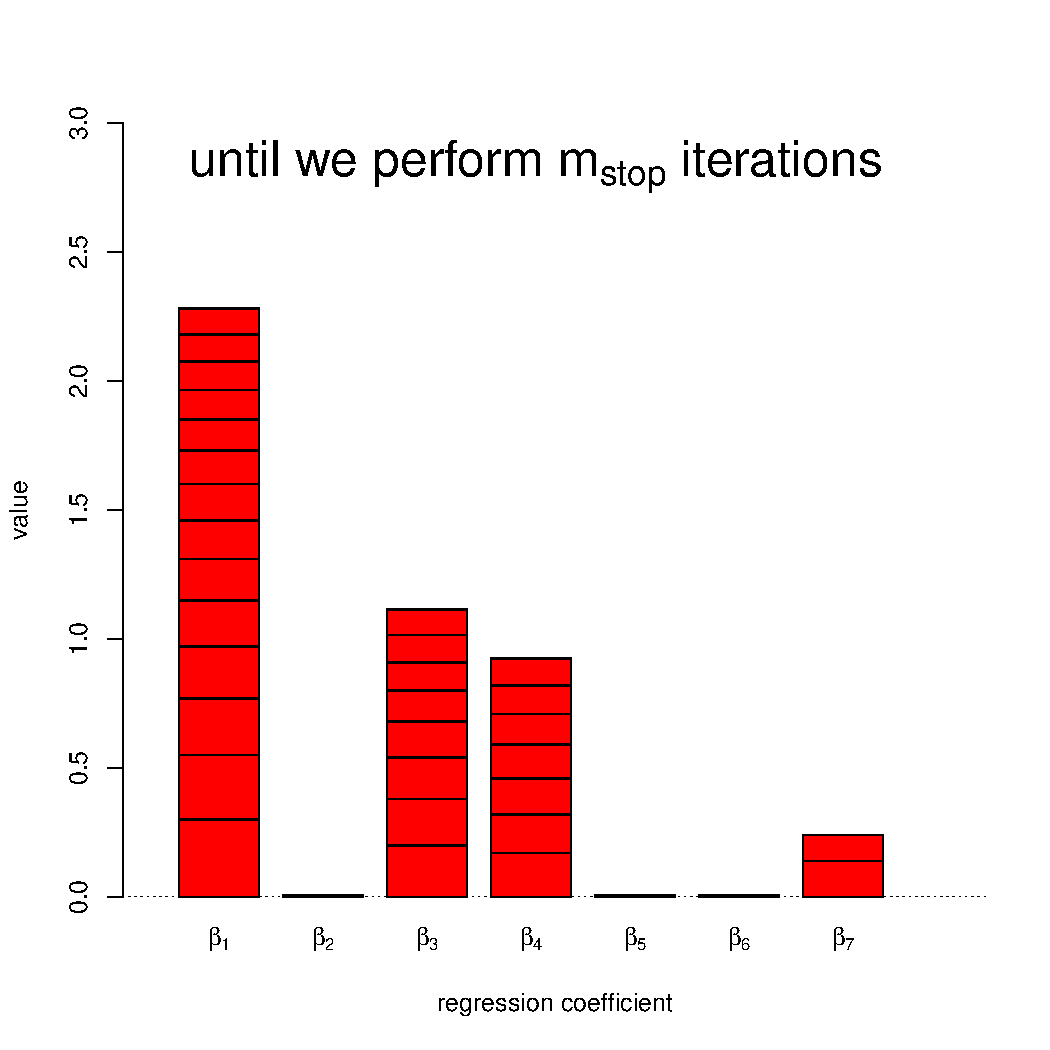
\includegraphics[width=0.75\textwidth]{figures/boosting_9}
\end{figure}
}

\frame{\frametitle{Boosting: }
\framesubtitle{tuning parameters}
\begin{itemize}
  \item The update step is regulated by the \textcolor{uio}{shrinkage parameter $\nu$};
  \item as long as its \textcolor{uio}{magnitude is reasonable}, the choice of the penalty parameter does \textcolor{uio}{not} influence the procedure;
\end{itemize}

\vspace{-1pt}

\begin{itemize}
  \item the choice of the \textcolor{uio}{number of iterations $m_{stop}$} is highly relevant;
  \item $m_{stop}$ (complexity parameter) influences \textcolor{uio}{variable selection properties} and model sparsity;
  \item $m_{stop}$ controls the amount of \textcolor{uio}{shrinkage};
   \begin{itemize}
      \item $m_{stop}$ \textcolor{uio}{too small} results in a model which is \textcolor{uio}{not able} to describe the data variability;
      \item an \textcolor{uio}{excessively large} $m_{stop}$ causes \textcolor{uio}{overfitting} and causes the selection of irrelevant variables.
    \end{itemize}
\end{itemize}

\vspace{-1pt}

\begin{itemize}
  \item there is no standard approach $\rightarrow$ \textcolor{uio}{repeated cross-validation} \citep{SeiboldAl2016}.
\end{itemize}
}


\section{Likelihood-based Boosting}

\subsection{introduction}

\frame{\frametitle{Likelihood-based Boosting: }
\framesubtitle{introduction}
A different version of boosting is the so-called {\bf \uline{likelihood-based boosting}} \citep{TutzBinder2006}:
\begin{itemize}
\item based on the concept of \textcolor{uio}{GAM} as well;
\item loss function as a \textcolor{uio}{negative log-likelihood};
\item uses standard statistical tools (\textcolor{uio}{Fisher scoring}, basically a Newton-Raphson algorithm) to minimize the loss function;
\item likelihood-based boosting and gradient boosting are \textcolor{uio}{equal only in Gaussian} regression \citep{Debin2016a}.
\end{itemize}
}

\frame{\frametitle{Likelihood-based Boosting: }
\framesubtitle{algorithm}
The simplest implementation of the likelihood-based boosting is \textcolor{uio}{BoostR}, based on the ridge estimator:

\vspace{6pt}

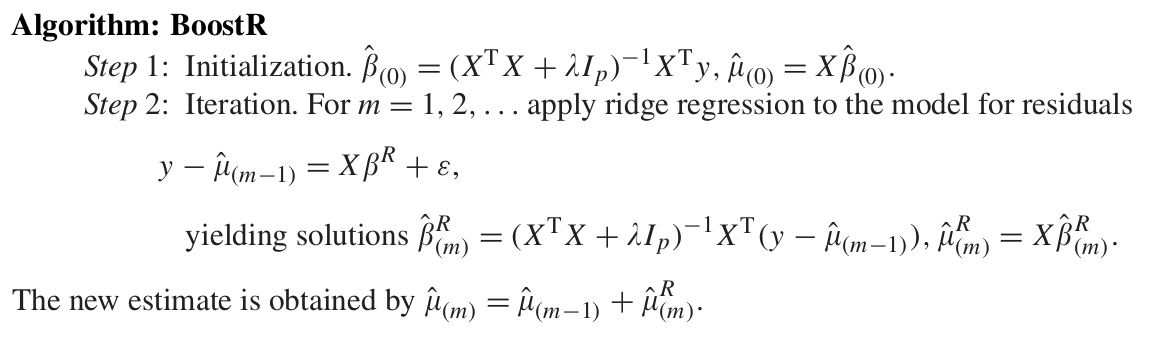
\includegraphics[width=\textwidth]{BoostR}

see also \cite{TutzBinder2007}.

\vspace{6pt}

In the rest of the lecture we will give the \textcolor{uio}{general idea} and see its implementation as a special case of gradient boosting.
}

\frame{\frametitle{Likelihood-based Boosting: }
\framesubtitle{introduction}
\begin{columns}
\begin{column}{0.75\textwidth}
\vspace{-0.75cm}
\begin{figure}
  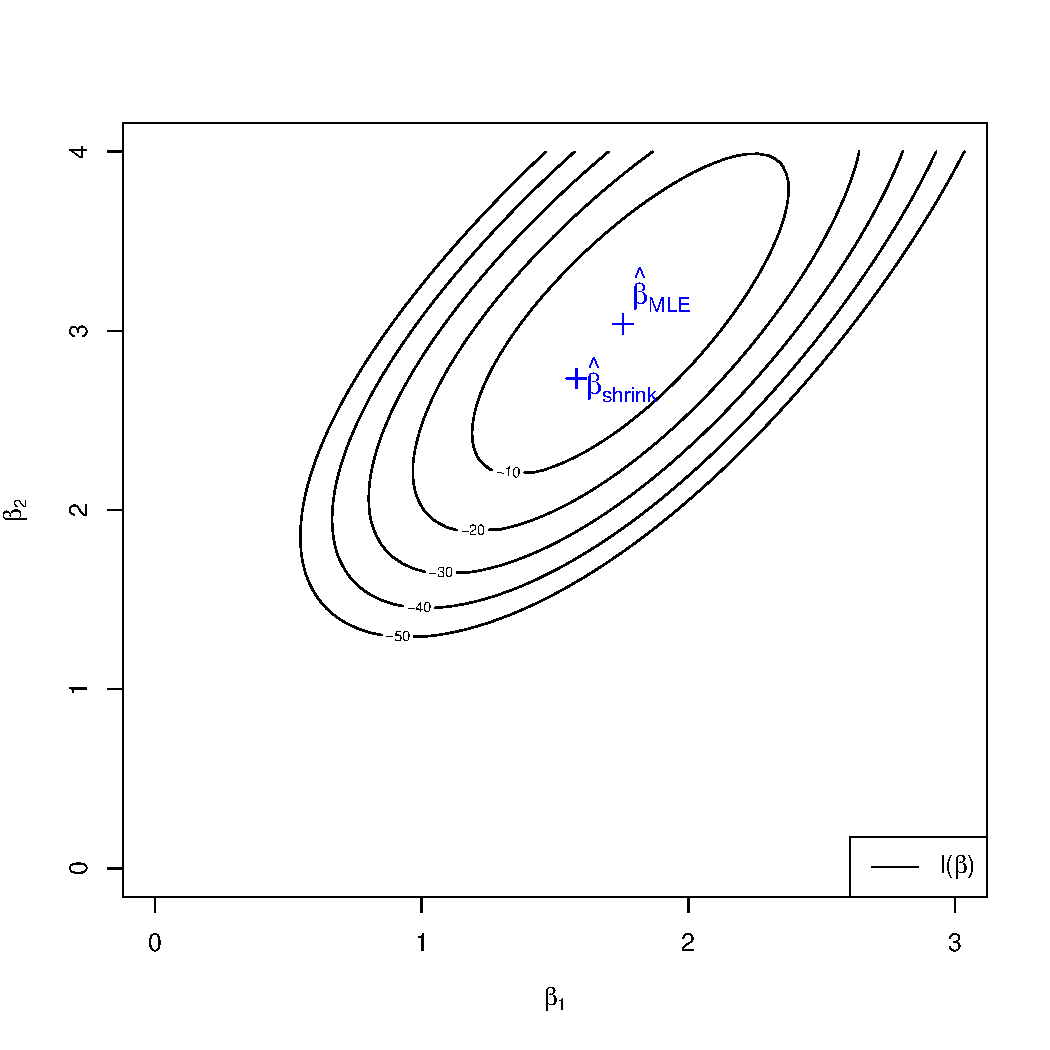
\includegraphics[width=\textwidth]{figures/fig1}
\end{figure}
\end{column}
\begin{column}{0.5\textwidth}
Following the statistical interpretation of boosting:\\

\vspace{0.5cm}
maximize the\\
\textcolor{uio}{log-likelihood} $\ell(\beta)$\\
(equivalently, $-\ell(\beta)$ is the \\ \textcolor{uio}{loss function} to minimize);

\vspace{0.5cm}
prediction $\rightarrow$ \textcolor{uio}{shrinkage}\\
aim at \textcolor{uio}{$\hat{\beta}_{shrink}$}, not $\hat{\beta}_{MLE}$;\\

\vspace{0.5cm}
best solution is ``between''\\ 0 and $\hat{\beta}_{MLE}$.

\end{column}
\end{columns}
}


\frame{\frametitle{Likelihood-based Boosting: }
\framesubtitle{introduction}
\begin{columns}
\begin{column}{0.75\textwidth}
\vspace{-0.75cm}
\begin{figure}
  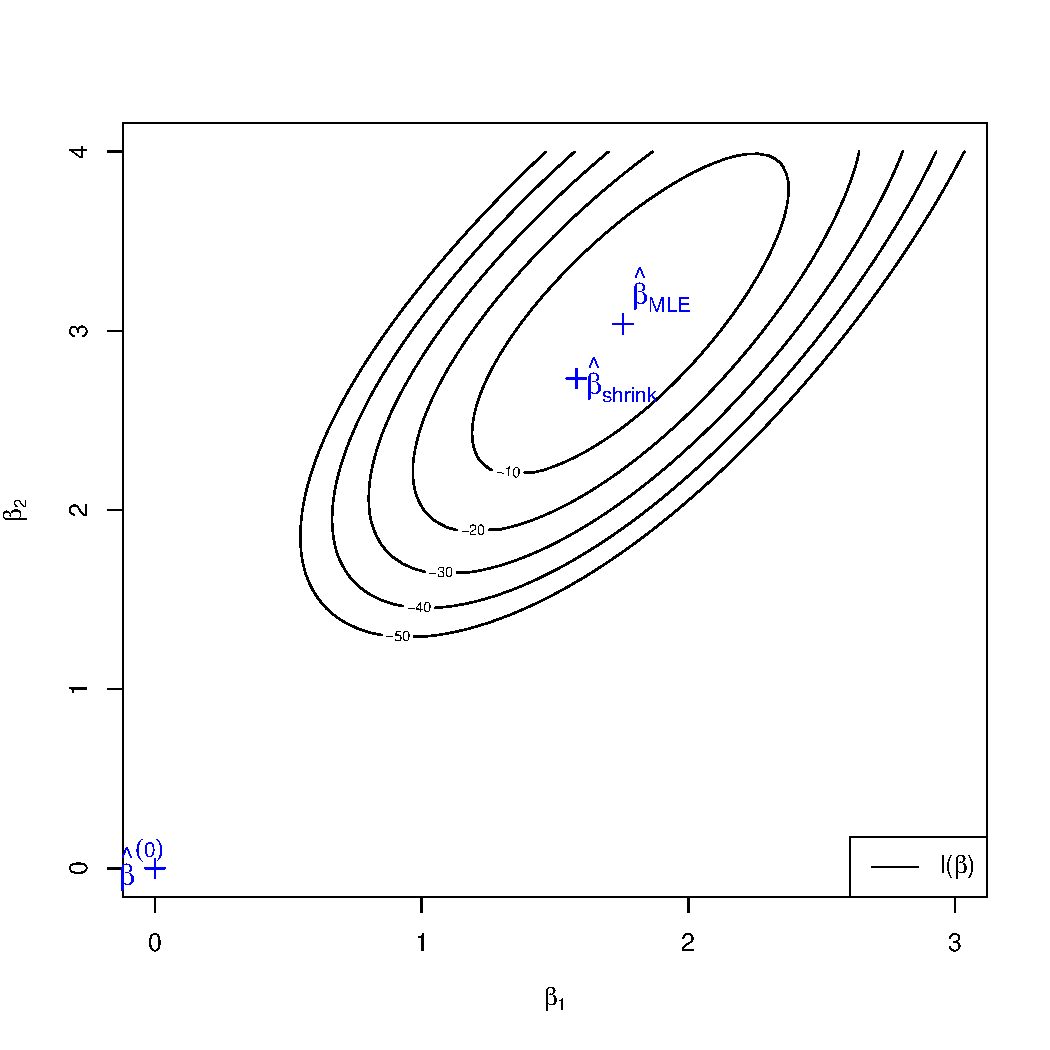
\includegraphics[width=\textwidth]{figures/fig2}
\end{figure}
\end{column}
\begin{column}{0.5\textwidth}

starting point...\\
maximize a log-likelihood...

\begin{center}
\hspace{-1.5cm}
$\Downarrow$
\end{center}

\textcolor{uio}{Newton-Raphson} method \\
(or Fisher scoring).

\vspace{0.5cm}
Basic idea:\\
- apply Newton-Raphson;\\
- stop early enough to end\\ in $\hat{\beta}_{shrink}$ and not in $\hat{\beta}_{MLE}$.

\end{column}
\end{columns}

}


\frame{\frametitle{Likelihood-based Boosting: }
\framesubtitle{Newton-Raphson}
General Newton-Raphson step:
$$
\hat{\beta}^{[m]} = \hat{\beta}^{[m-1]} + \left(\left. -\ell_{\beta\beta}(\beta)\right|_{\beta=\hat{\beta}^{[m-1]}}\right)^{-1}\left.\ell_\beta(\beta)\right|_{\beta=\hat{\beta}^{[m-1]}},
$$
where:
\begin{itemize}
\item $\ell_{\beta}(\beta)=\frac{\partial \ell(\beta)}{\partial \beta}$;
\item $\ell_{\beta\beta}(\beta)=\frac{\partial^2 \ell(\beta)}{\partial \beta^T \partial \beta}$.
\end{itemize}

For convenience, let us rewrite the general step as
$$
\underbrace{\hat{\beta}^{[m]} - \hat{\beta}^{[m-1]}}_\text{improvement at step $m$} = 0 + \left(\left. -\ell_{\beta\beta}(\beta|\hat{\beta}^{[m-1]})\right|_{\beta=0}\right)^{-1}\left.\ell_\beta(\beta|\hat{\beta}^{[m-1]})\right|_{\beta=0}.
$$

}


\frame{\frametitle{Likelihood-based Boosting: }
\framesubtitle{Newton-Raphson}
Control the Newton-Raphson algorithm:
\begin{itemize}
\item we need to force the estimates to be \textcolor{uio}{between 0 and $\hat{\beta}_{MLE}$};
\item we need to \textcolor{uio}{be able to stop at $\hat{\beta}_{shrink}$}.
\item[$\Rightarrow$] we need smaller ``controlled'' improvements.
\item[]
\end{itemize}

\vspace{-0.3cm}
Solution: \textcolor{uio}{penalize the log-likelihood}!
\begin{itemize}
\item $p\ell(\beta) \leftarrow \ell(\beta) - \frac{1}{2}\lambda ||\beta||_2^2$;
\item $p\ell_{\beta}(\beta) \leftarrow \ell_{\beta}(\beta) - \lambda ||\beta||_1$;
\item $p\ell_{\beta\beta}(\beta) \leftarrow \ell_{\beta\beta}(\beta) - \lambda$;
\item[]
\end{itemize}

\vspace{-0.3cm}
Now the general step is:
$$
\underbrace{\hat{\beta}^{[m]} - \hat{\beta}^{[m-1]}}_\text{improvement at step $m$} = \left(\left. -\ell_{\beta\beta}(\beta|\hat{\beta}^{[m-1]})\right|_{\beta=0} + \lambda\right)^{-1}\left.\ell_\beta(\beta|\hat{\beta}^{[m-1]})\right|_{\beta=0}
$$
}


\frame{\frametitle{Likelihood-based Boosting: }
\framesubtitle{visualization}
\begin{columns}
\begin{column}{0.75\textwidth}
\vspace{-0.75cm}
\begin{figure}
  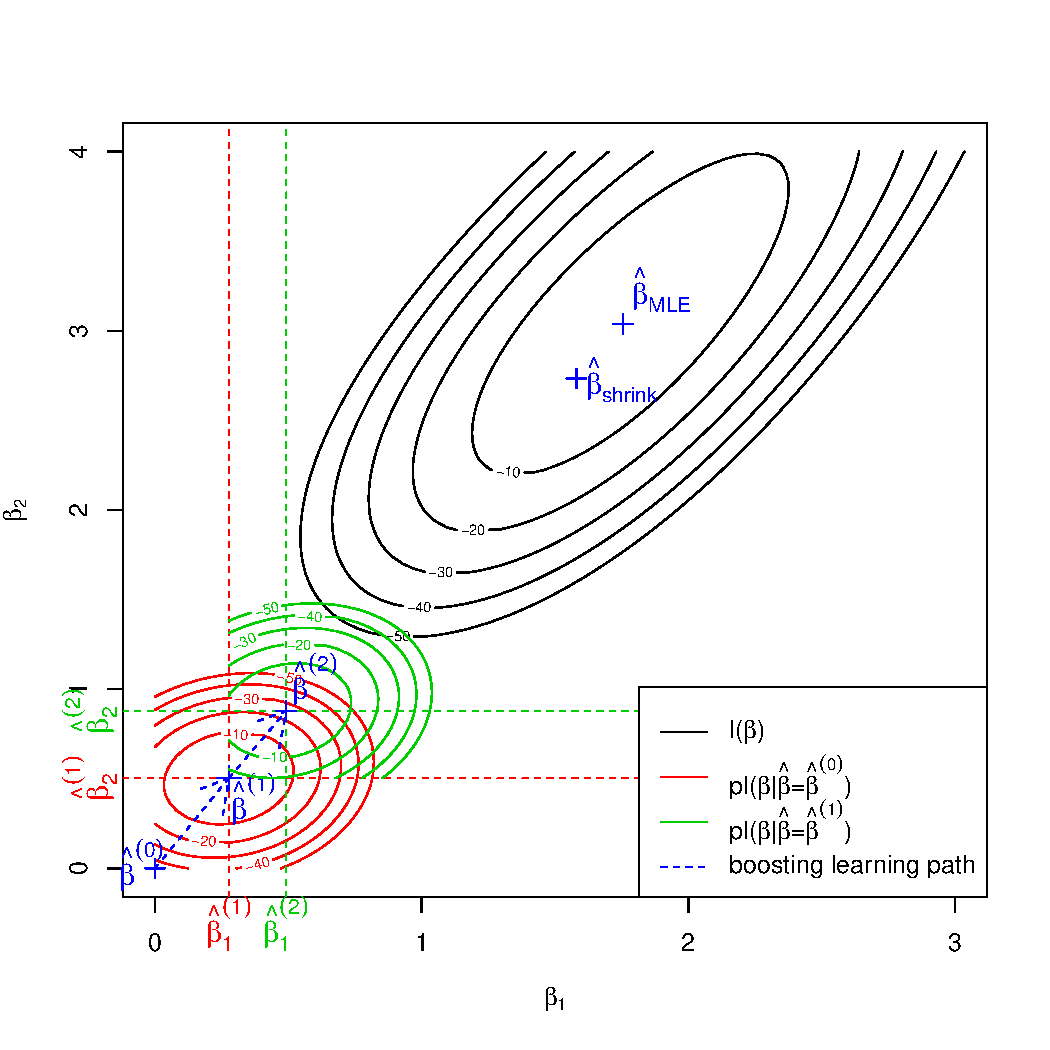
\includegraphics[width=\textwidth]{figures/boostingRR2}
\end{figure}
\end{column}
\begin{column}{0.5\textwidth}

As long as \textcolor{uio}{$\lambda$ is `big enough'},\\
the boosting learning path\\
is going to hit $\hat{\beta}_{shrink}$.

\vspace{0.5cm}
We \textcolor{uio}{must stop} at that point:\\
the number of boosting\\
iterations (\textcolor{uio}{$m_{stop}$}) is crucial!

\end{column}
\end{columns}
}


\frame{\frametitle{Likelihood-based Boosting: }
\framesubtitle{likelihood-based vs gradient}
In the \textcolor{uio}{likelihood-based boosting} we:
\begin{itemize}
\item \textcolor{uio}{repeatedly} implement the first step of \textcolor{uio}{Newton-Raphson};
\item \textcolor{uio}{update} at each step \textcolor{uio}{estimates} and likelihood.
\item[]
\end{itemize}

Small improvements:
\begin{itemize}
  \item \textcolor{uio}{parabolic approximation};
  \item fit the \textcolor{uio}{negative gradient} on the data by a base-learner (e.g., least-square estimator)
  $$
\hat{\beta}^{[m]} - \hat{\beta}^{[m-1]} = \left(X^TX + \lambda\right)^{-1}X^T \underbrace{\left.\frac{\partial \ell(\eta(\beta,X))}{\partial \eta(\beta,X)}\right|_{\hat{\beta}^{[m-1]}}}_\text{negative gradient}
$$
\end{itemize}
}


\frame{\frametitle{Likelihood-based Boosting: }
\framesubtitle{likelihood-based vs gradient}
Substituting
$$
\nu=\left(X^T X+\lambda\right)^{-1} X^TX
$$
one obtains the expression of the \textcolor{uio}{$L_2$Boost} for (generalized) linear models seen before,
$$
\hat{\beta}^{[m]} - \hat{\beta}^{[m-1]} = \nu \left(X^TX\right)^{-1}X^T \left.\frac{\partial \ell(\eta(\beta,X))}{\partial \eta(\beta,X)}\right|_{\hat{\beta}^{[m-1]}}
$$

\begin{itemize}
\item \textcolor{uio}{gradient boosting} is a \textcolor{uio}{much more general} algorithm;
\item likelihood-based boosting and gradient boosting are \textcolor{uio}{equal in Gaussian} regression because the log-likelihood is a parabola;
\item both have a \textcolor{uio}{componentwise version}.
\end{itemize}
}


\frame{\frametitle{Likelihood-based Boosting: }
\framesubtitle{likelihood-based vs gradient}
Alternatively (more correctly) we can see the likelihood-based boosting as a special case of the gradient boosting \citep{Debin2016a}:
\begin{enumerate}
  \item initialize $\hat{\beta}=(0,\dots,0)$;
  \item for $m = 1, \dots, m_\text{stop}$
  \begin{itemize}
  \item compute the negative gradient vector, $u=\left.\frac{\partial \ell(f(x,\beta))}{\partial f(x,\beta)}\right|_{\beta=\hat{\beta}}$
  \item compute the update,
	\vspace{-0.4cm}
	\textcolor{uio}{$$
	\hat{b}^{LB} = \left(\left.\frac{\partial f(x,\beta)}{\partial \beta}\right|_{\beta=0}^\top u \right) / \left(-\left.\frac{\partial \frac{\partial f(x,\beta)}{\partial \beta}}{\partial \beta}\right|_{\beta=0}^\top u+\lambda\right);
	$$}
  \item update the estimate, $\hat{\beta}^{[m]} = \hat{\beta}^{[m-1]} + \hat{b}^{LB}$.
  \end{itemize}
  \item compute the final prediction, e.g., for lin.\ regr.\ $\hat{y} = X^T\hat{\beta}^{[m_\text{stop}]}$
\end{enumerate}
}


\section{Tree-based boosting}

\frame{\frametitle{Tree-based boosting: }
\framesubtitle{introduction}
The \textcolor{uio}{base (weak) learner} in a boosting algorithm can be a \textcolor{uio}{tree}:
\begin{itemize}
\item largely used in practice;
\item very \textcolor{uio}{powerful and fast} algorithm;
\item R package \textcolor{uio}{\texttt{XGBoost}};
\item we \textcolor{uio}{lose part} of the statistical interpretation.
\end{itemize}
}


\frame{\frametitle{Tree-based boosting: }
\framesubtitle{algorithm}
\centering
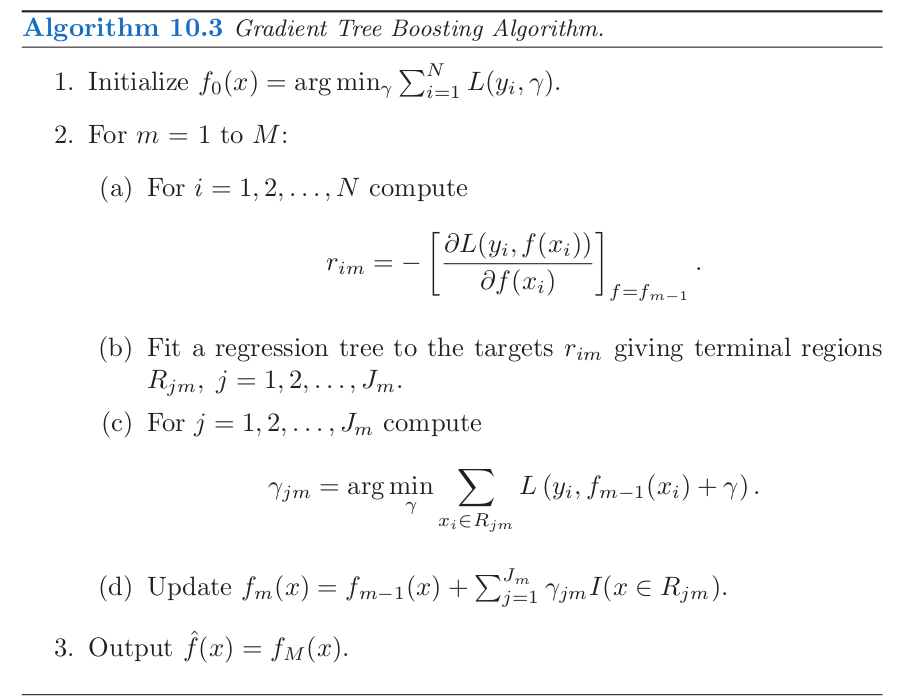
\includegraphics[width=0.9\textwidth]{alg10_3}
}


\frame{\frametitle{Tree-based boosting: }
\framesubtitle{importance of ``weakness''}
\centering
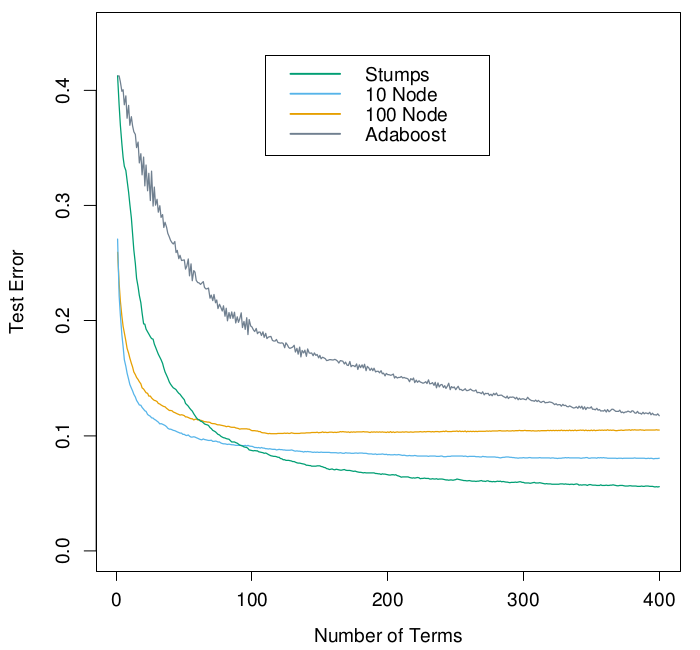
\includegraphics[width=0.75\textwidth]{fig10_9}
}


\frame{\frametitle{Tree-based boosting: }
\framesubtitle{importance of ``shrinkage''}
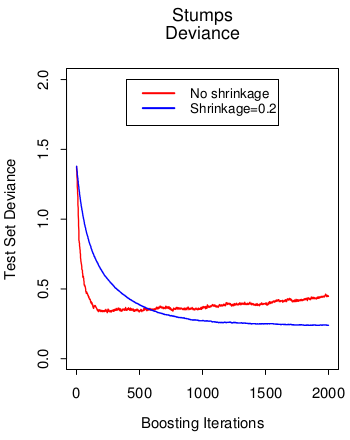
\includegraphics[width=0.5\textwidth]{fig10_11_tl}
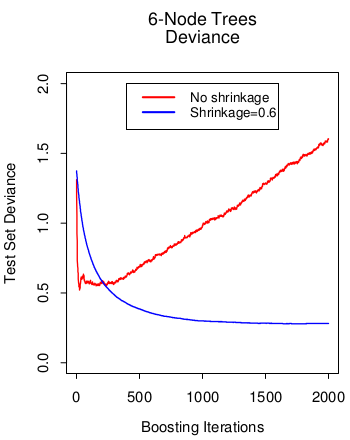
\includegraphics[width=0.5\textwidth]{fig10_11_bl}
}


\frame{\frametitle{Tree-based boosting: }
\framesubtitle{comparison}
\centering
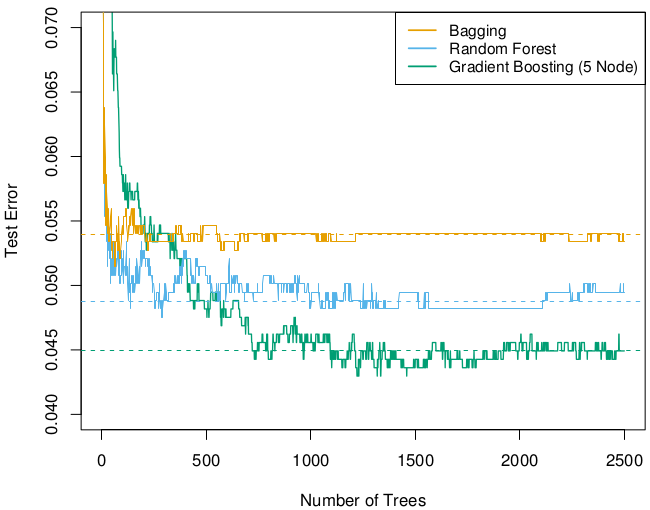
\includegraphics[width=0.9\textwidth]{fig15_1}
}



%%%%%%%%%%%
\section*{Bibliography}
%%%%%%%%%%%

\frame[allowframebreaks]{\frametitle{References}
\footnotesize
\bibliographystyle{../../../../support/biometrika}
\bibliography{../../../../support/biblio}
}

\end{document}
